\documentclass{bioinfo}
\copyrightyear{2015}
\pubyear{2015}

\usepackage{url}
\usepackage{color}

%\newcommand{\co}[1]{}
\newcommand{\co}[1]{[{\color{red} #1}]}
\newcommand{\coout}[1]{}

\begin{document}
\firstpage{1}

\title[Parameter balancing]{Parameter balancing: consistent parameter sets for kinetic metabolic models}
\author[Lubitz \textit{et~al}]{Timo Lubitz\,$^{1}$ and Wolfram Liebermeister\,$^{2,3}$\footnote{to whom correspondence should be addressed}}
\address{$^{1}$Theoretische  Biophysik, Institut f\"ur  Biologie, Humboldt-Universit\"at zu Berlin, Berlin, Germany \\
$^{2}$INRA, UR1404, MaIAGE, Universit\'e Paris-Saclay, Jouy-en-Josas, France\\
$^{3}$Institut f\"ur Biochemie, Charit\'e -- Universit\"atsmedizin Berlin, Berlin, Germany
}

\history{Received on XXXXX; revised on XXXXX; accepted on XXXXX}

\editor{Associate Editor: XXXXXXX}

\maketitle


\begin{abstract}
\section{Summary:}
Parameter balancing is a Bayesian method to determine consistent parameter sets for metabolic models. Incomplete, uncertain kinetic data are translated into balanced parameter sets, which are complete and thermodynamically consistent. Thermodynamic and metabolomic data can also be balanced, yielding feasible metabolic states. Aside from point estimates, uncertainty ranges and correlations of the variables in question can be determined. We provide  online  and command line tools for Parameter Balancing, as well as Python and Matlab implementations.  The tools use standard model and data formats. Prior information about biochemical constants is freely customisable by the user.

\section{Availability and Implementation:}
Online services, code, and documentation are accessible at
\url{www.parameterbalancing.net}. Code includes a command line tool, a
Python package and a Matlab toolbox.

\section{Supplementary Information:}
Documentation and example models can be found at \url{www.parameterbalancing.net}. 


\section{Contact:} wolfram.liebermeister@gmail.com, timo.lubitz@gmail.com
\end{abstract}

\section{Introduction}

Kinetic modelling is a common approach to studying the metabolic
dynamics of cells. One of the main challenges in model construction is
the choice of rate laws and kinetic parameters such as
Michaelis-Menten constants, catalytic rate constants, or equilibrium
constants. Kinetic and thermodynamic constants have been collected in
repositories such as BRENDA (\cite{scheer2010brenda}), eQuilibrator
(\cite{flamholz2011equilibrator}), or SABIO-RK
(\cite{wittig2011sabio}), and kinetic metabolic models can be
populated automatically with kinetic rate laws
\cite{likl:06a,dhss:08}.  However, when inserting measured parameter
values directly into a model, many model parameters may remain
undetermined or may even be inconsistent. Typically, various
parameters have not been measured or carry large experimental
uncertainties (due to \emph{in-vitro} measurements, measurements in
different model organisms, and different experimental
setups). Moreover, enzyme parameters can be physically dependent
because of thermodynamic Wegscheider conditions and Haldane
relationships (\cite{haldane1930enzymes}). Ignoring these dependencies
can lead to thermodynamically incorrect models showing a
\emph{perpetuum mobile}-like behaviour. In principle, missing
parameters can be determined by fitting a model to metabolomic
time-series data (for a review, see
\cite{ashyraliyev2009systems}). For larger models, however, model
fitting becomes numerically hard, parameters may not be identifiable,
and in practice thermodynamic dependencies between parameters are
often ignored.

Parameter balancing (\cite{lubitz2010parameter}) addresses these
problems by converting measured kinetic constants into complete,
consistent sets of model parameters. It accounts for dependencies
between kinetic constants arising from their definition or
thermodynamic laws (such as the Wegscheider conditions and Haldane
relationships) and uses these dependencies to improve the calculation
of mean values, uncertainties, and correlations between the parameters
in question. Prior distributions are used to keep parameter values in
reasonable ranges. Given the model’s network structure, measured
kinetic parameters, and prior distributions for the kinetic constants,
parameter balancing determines a multivariate posterior distribution
describing all model parameters. Point estimates and uncertainty
ranges for individual model parameters can be extracted from the
posterior, and consistent parameter sets can be sampled to create a
model ensemble representing the range of possible models compatible
with available data. Each of the sampled models and metabolic states
is thermodynamically consistent. Aside from kinetic constants, the
method can also be applied to determine feasible metabolic states,
characterised by metabolite concentrations and thermodynamic forces.

\section{Results and Implementation}

Parameter balancing helps modellers determine consistent kinetic
parameter sets for metabolic models.  We have implemented the
parameter balancing algorithm as a Python package and provide a
convenient online interface. While the online interface enables the
user to perform parameter balancing with default configuration with a
few mouse clicks, users can embed the Python code into their own
modelling workflows (\cite{stanford2013systematic}). Based on a
metabolic network model and a (possibly incomplete) set of kinetic
constants, a table with balanced model parameters is computed. Using
these model parameters a kinetic model with modular rate laws
(\cite{liebermeister2010modular}) in the standard format SBML is
generated. The simple default usage can be extended by using various
configuration options. We defined biologically plausible priors for
different types of kinetic constants.  Instead of using these default
priors, users can define their own customized priors be specifying
geometric mean values, geometric standard deviations, and feasible
ranges. To make the method widely applicable, we sought to support
established standard formats: models are provided in SBML (Systems
Biology Markup Language) format (\cite{hucka2003systems}), and all other data are
given in the table format SBtab (\cite{lubitz2016sbtab}).


\begin{figure}[t]
\begin{center}
 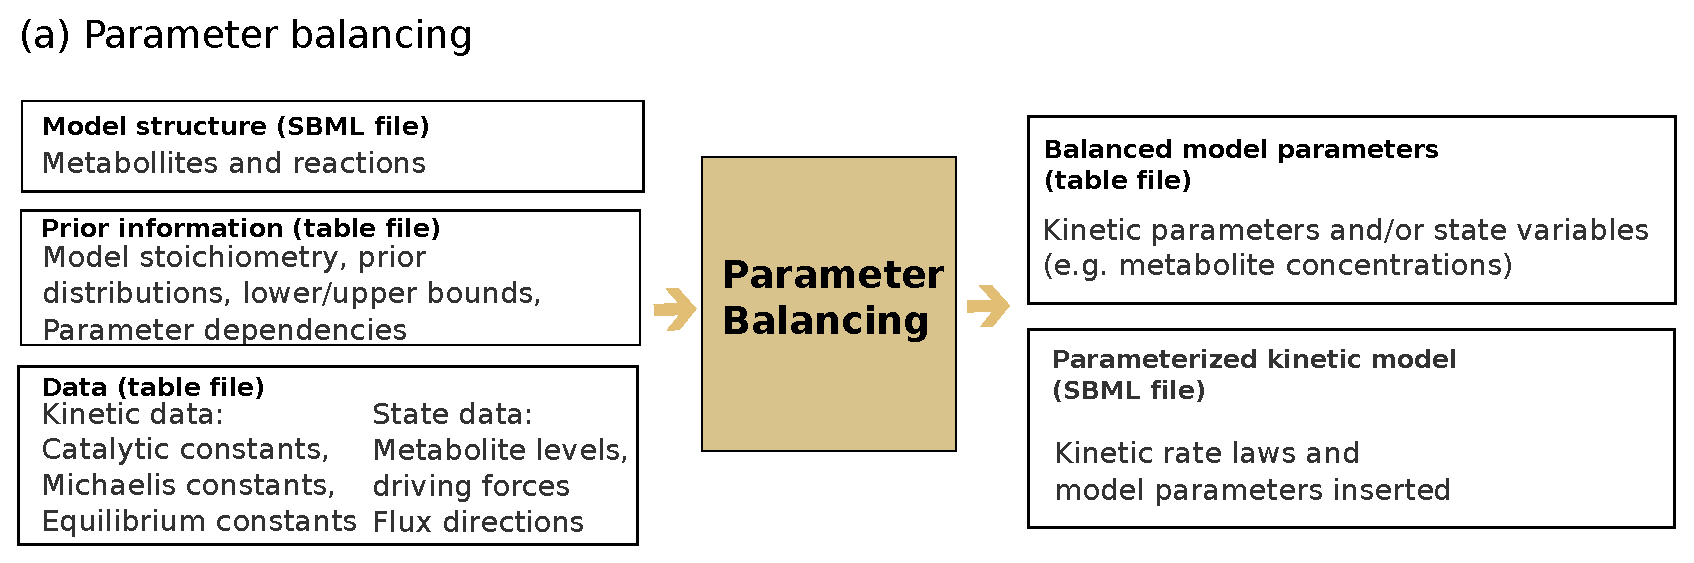
\includegraphics[width=0.49\textwidth]{figures/workflow.eps}\\[2mm]
 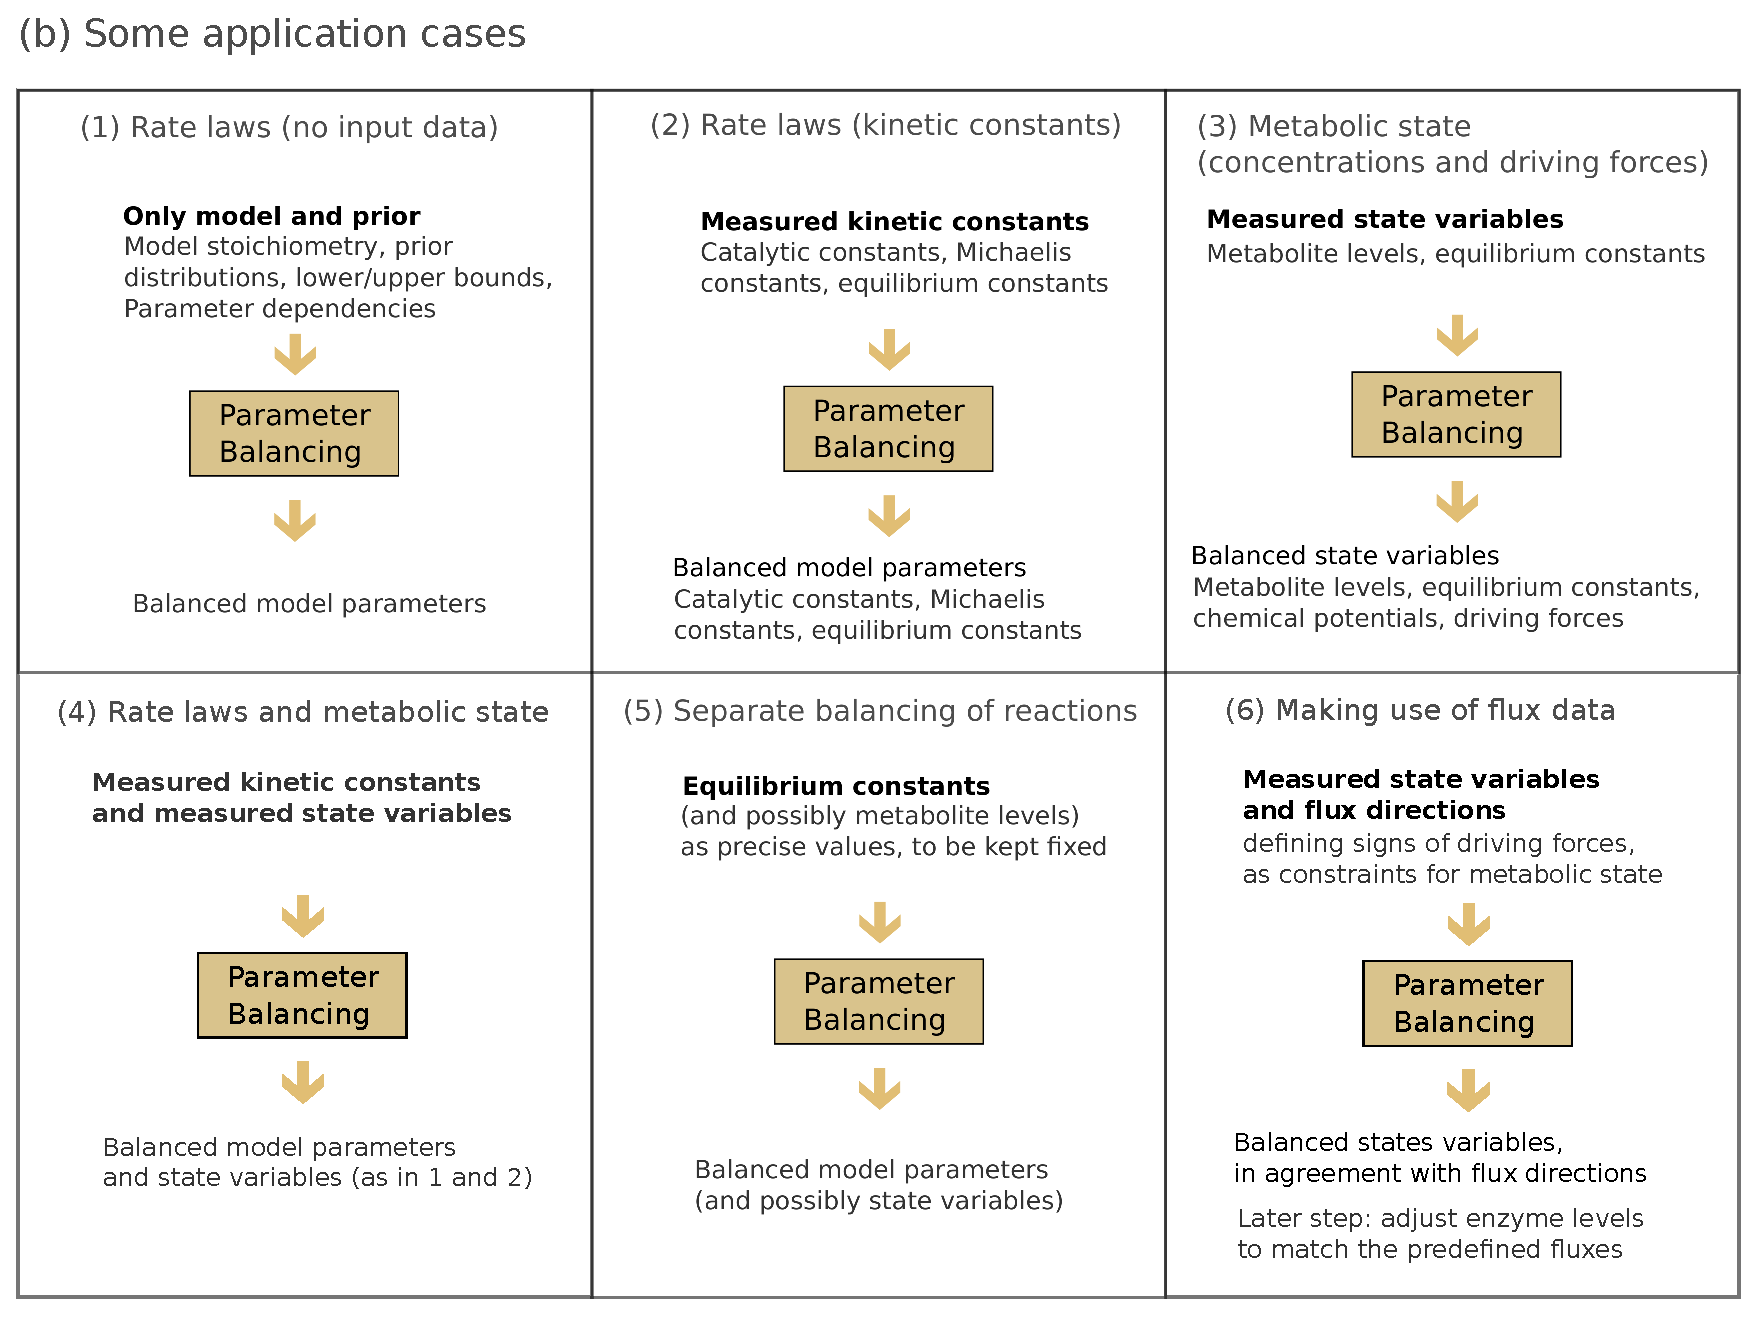
\includegraphics[width=0.49\textwidth]{figures/scenarios.eps}
 \caption[Parameter balancing]{Potential usage scenarios for parameter balancing: (1) Converting incomplete kinetic data and equilibrium constants into a balanced set of kinetic model parameters. (2) Providing metabolite levels and equilibrium constants to determine reasonable metabolic states (i.e. metabolite levels, equilibrium constants, chemical potentials, and thermodynamic forces). (3) Combining (1) and (2) for metabolic state, balanced kinetic constants, and rate laws. (4) Finding reasonable kinetic parameters for a given model stoichiometry; kinetic constant are determined from prior distributions, upper and lower bounds, and mutual parameter dependencies. (5) To simplify the calculations, parameters may be balanced separately in each reaction. In this variant of the method, equilibrium constants and metabolite levels need to be fixed to avoid inconsistencies in the resulting model. (6) If metabolic fluxes are known, the flux directions can be used to narrow down the possible metabolic states. After parameter balancing, the enzyme levels can be adjusted to match the predefined fluxes.
 \vspace{-5mm}
\label{ParameterBalancing}}
\end{center}
\end{figure}

\section{Conclusion}

Parameter balancing allows modellers to translate a metabolic network
into a simulatable dynamic model almost automatically. It can be
integrated into modelling workflows with different kinds of available
data and model parameters to be determined. As shown in Figure 1
(\ref{ParameterBalancing}), it can either be used to determine
plausible default parameters (without any data, and based on prior
distributions only), to balance a set of given kinetic constants, or
to determine thermodynamically consistent metabolic states (comprising
metabolite levels and thermodynamic forces, and accounting for known
flux directions). Parameter balancing can be applied to single
reactions or larger networks.  Experimental data - including
equilibrium constants, catalytic rate constants, Michaelis constants,
metabolite and enzyme concentrations - need to be collected from
literature and web resources. Adding more data will make the balanced
parameters more accurate and will decrease their uncertainty
ranges. Metabolic fluxes cannot be used directly as input data because
the kinetic rate laws do not fit into the regression model behind
parameter balancing. However, known flux directions can be used to
restrict the thermodynamic forces and to narrow down the possible
metabolite levels predicted by parameter balancing. The resulting
state can then be matched to the given fluxes by adjusting the enzyme
levels.  As a potential future application, the posterior
distributions obtained from parameter balancing could be used as
priors for subsequent rounds of model fitting
(\cite{liebermeister2006bringing}).

\paragraph{Acknowledgements}
The authors wish to thank Elad Noor for pleasant and insightful
discussions. \co{Natalie?  who else?} This work was generously
supported by the German Research Foundation (grant number Ll 1676/2-1
to WL). 
\vspace{-.5cm}

\ \\[-10mm]

\bibliographystyle{natbib}
\bibliography{references}



\end{document}
